% !TeX program = xelatex
% =====================================================================
%  pci_test command-line quick reference card
%  Engine : XeLaTeX  (xeCJK + TikZ + tcolorbox)
%  Build  : xelatex pci_test_refcard.tex   (run twice)
% =====================================================================
\documentclass[10pt,a4paper,landscape]{article}

\usepackage{geometry}
\geometry{a4paper,landscape,left=8mm,right=8mm,top=8mm,bottom=11mm}

\usepackage{fontspec}
\usepackage{xeCJK}
\usepackage{xcolor}
\usepackage{tikz}
\usetikzlibrary{positioning,calc,arrows.meta,shapes.geometric,decorations.pathreplacing}
\usepackage[most]{tcolorbox}
\usepackage{multicol}
\usepackage{enumitem}
\usepackage{fancyhdr}

% ---------------------------------------------------------------- fonts
\setmainfont{DejaVu Sans Condensed}
\setsansfont{DejaVu Sans Condensed}
\setmonofont{Liberation Mono}[Scale=0.94]
\setCJKmainfont{Noto Sans CJK SC}
\setCJKsansfont{Noto Sans CJK SC}
\setCJKmonofont{Noto Sans CJK SC}

% --------------------------------------------------------------- colors
\definecolor{cDev}  {HTML}{0F766E}   % teal   - device
\definecolor{cBar}  {HTML}{1D4ED8}   % blue   - BAR tasks
\definecolor{cBarP} {HTML}{0284C7}   % sky    - BAR params
\definecolor{cDma}  {HTML}{C2410C}   % orange - DMA tasks
\definecolor{cDmaP} {HTML}{B45309}   % amber  - DMA params
\definecolor{cNum}  {HTML}{7E22CE}   % purple - numeric mode
\definecolor{cWarn} {HTML}{B91C1C}   % red    - pitfalls
\definecolor{cEx}   {HTML}{15803D}   % green  - examples
\definecolor{cMisc} {HTML}{475569}   % slate  - misc
\definecolor{cInk}  {HTML}{1E293B}
\definecolor{cGrey} {HTML}{64748B}

% ------------------------------------------------------------ tcolorbox
\newtcolorbox{panel}[2]{%
  enhanced, breakable,
  colback=#1!4!white, colframe=#1!88!black,
  coltitle=white, colbacktitle=#1,
  boxrule=0.5pt, arc=2.5pt,
  left=3pt, right=3pt, top=3pt, bottom=3pt,
  toptitle=1.2pt, bottomtitle=1.2pt,
  fonttitle=\bfseries\small,
  before upper=\raggedright,
  title={#2}}

% -------------------------------------------------------------- macros
% coloured rounded badge for a short option (drawn with TikZ)
\newcommand{\badge}[2]{%
  \tikz[baseline=(bx.base)]{%
    \node[fill=#1,text=white,rounded corners=1.6pt,
          inner xsep=2.6pt,inner ysep=1.1pt,
          font=\ttfamily\bfseries](bx){#2};}}

% \cmdrow{colour}{short}{long}{argument}{description}
\newcommand{\cmdrow}{\begingroup\catcode`\_=12\relax\cmdrowaux}
\newcommand{\cmdrowaux}[5]{%
  \par\vspace{1.6pt}\noindent
  \badge{#1}{#2}\hspace{2.6pt}%
  {\ttfamily\color{#1!75!black}#3}%
  \ifx\relax#4\relax\else\hspace{2.6pt}{\itshape\color{cGrey}#4}\fi
  \par\nobreak\vspace{0.4pt}%
  {\leftskip=1.5em\scriptsize\color{cInk}#5\par}%
  \endgroup}

% \prow{colour}{short}{long}{argument}{default}{description}
\newcommand{\prow}{\begingroup\catcode`\_=12\relax\prowaux}
\newcommand{\prowaux}[6]{%
  \par\vspace{1.6pt}\noindent
  \badge{#1}{#2}\hspace{2.6pt}%
  {\ttfamily\color{#1!75!black}#3}%
  \ifx\relax#4\relax\else\hspace{2.6pt}{\itshape\color{cGrey}#4}\fi
  \ifx\relax#5\relax\else\hspace{2.6pt}%
    \tikz[baseline=(df.base)]{\node[draw=#1!45,fill=#1!8,rounded corners=1.4pt,
      inner xsep=2.2pt,inner ysep=0.8pt,font=\scriptsize](df){默认 #5};}\fi
  \par\nobreak\vspace{0.4pt}%
  {\leftskip=1.5em\scriptsize\color{cInk}#6\par}%
  \endgroup}

% \testrow{id}{title}{positional arguments}
\newcommand{\testrow}{\begingroup\catcode`\_=12\relax\testrowaux}
\newcommand{\testrowaux}[3]{%
  \par\vspace{1.8pt}\noindent
  \tikz[baseline=(tid.base)]{%
    \node[circle,fill=cNum,text=white,inner sep=0pt,minimum size=3.6mm,
          font=\bfseries\scriptsize](tid){#1};}\hspace{3pt}%
  {\bfseries\small\color{cNum!70!black}#2}%
  \par\nobreak\vspace{0.4pt}%
  {\leftskip=1.6em\scriptsize\ttfamily\color{cInk}#3\par}%
  \endgroup}

% single shell line, verbatim-ish
\newcommand{\shell}{\begingroup\catcode`\_=12\catcode`\$=12\relax\shellaux}
\newcommand{\shellaux}[1]{%
  \par\vspace{0.6pt}\noindent
  {\ttfamily\scriptsize\color{cEx!55!black}\$\ }%
  {\ttfamily\scriptsize\color{cInk}#1}\par\endgroup}

% inline literal with free underscores
\newcommand{\lit}{\begingroup\catcode`\_=12\relax\litaux}
\newcommand{\litaux}[1]{{\ttfamily #1}\endgroup}

% one row of the DMA address map: fixed column widths keep every bar the same
% size, so the bars can simply be stacked with below=of and need no coordinates
\newcommand{\dmarow}[2]{%
  \begin{tabular}{@{}p{10mm}@{}p{34mm}@{}p{11mm}@{}}
    \bfseries #1 & \ttfamily #2 & \raggedleft 4 GiB
  \end{tabular}}

% small caption line inside a panel
\newcommand{\note}[1]{\par\vspace{1.6pt}{\scriptsize\color{cGrey}#1}\par}
\newcommand{\sep}{\par\vspace{2pt}\noindent\textcolor{cGrey!40}{\rule{\linewidth}{0.3pt}}\par\vspace{1pt}}

% ------------------------------------------------------------- headers
\pagestyle{fancy}
\fancyhf{}
\renewcommand{\headrulewidth}{0pt}
\renewcommand{\footrulewidth}{0.3pt}
\fancyfoot[L]{\scriptsize\color{cGrey}pci\_test 命令行速查卡\quad|\quad Googoltech PCIe 驱动测试工具}
\fancyfoot[R]{\scriptsize\color{cGrey}第 \thepage\ 页}

\setlength{\parindent}{0pt}
\setlength{\columnsep}{5mm}
\setlength{\columnseprule}{0.3pt}
\renewcommand{\columnseprulecolor}{\color{cGrey!30}}

\begin{document}
\footnotesize

% =====================================================================
%  TITLE BANNER
% =====================================================================
\begin{tikzpicture}[node distance=1.5mm and 4mm]
  % the plate is the only sized element; everything else hangs off its anchors
  \node[rectangle, fill=cInk, rounded corners=3pt, inner sep=0pt,
        minimum width=\linewidth, minimum height=15.5mm] (plate) {};

  % accent stripe along the left edge of the plate
  \draw[cBar, line width=1.6mm, line cap=butt]
        ([xshift=0.8mm]plate.north west) -- ([xshift=0.8mm]plate.south west);

  \node[below right=2.2mm and 5mm of plate.north west, anchor=north west,
        text=white, font=\bfseries\Large] (title) {pci\_test 命令行速查卡};
  \node[below=of title.south west, anchor=north west, text=white!65, font=\scriptsize]
       {Googoltech PCIe 驱动（GOOGOL\_PCIe）用户态测试工具\ \ ·\ \ pci\_test\_amd64 / \_i386 / \_aarch64\ \ ·\ \ /opt/googoltech/bin/};

  \node[below left=3mm and 5mm of plate.north east, anchor=north east,
        text=white, font=\ttfamily\small] (cnt) {43 个选项};
  \node[below=of cnt.south east, anchor=north east, text=white!65, font=\ttfamily\scriptsize]
       {17 个测试编号};
\end{tikzpicture}

\vspace{2mm}

% =====================================================================
%  TWO INVOCATION MODES  (full width TikZ diagram)
% =====================================================================
\begin{tikzpicture}[font=\scriptsize, node distance=3mm and 6mm,
    box/.style={rectangle,rounded corners=2.5pt,draw=#1,fill=#1!7,
                text=cInk,inner xsep=4pt,inner ysep=3.5pt,align=left}]

  % anchor of the whole diagram: the upper branch box
  \node[box=cNum,text width=0.44\linewidth] (num)
       {\textcolor{cNum}{\bfseries 编号模式}\quad\textit{argv[1] 是纯数字，或完全不带参数}\\[1pt]
        \ttfamily pci\_test <IO\_DEV\_ID> <DMA\_DEV\_ID> <TEST\_ID> [位置参数...]\\[1pt]
        设备用\textbf{扫描序号}（非路径）\ \ ·\ \ 参数缺失时交互提问\ \ ·\ \ 详见「编号模式」区块};

  \node[box=cBar,text width=0.44\linewidth,
        below=of num.south west, anchor=north west] (opt)
       {\textcolor{cBar}{\bfseries 选项模式}\quad\textit{其余情况（以 - 开头）}\\[1pt]
        \ttfamily pci\_test [设备选项] [任务] [任务参数]\\[1pt]
        \lit{-d} / \lit{-D} \textbf{至少给一个}（完整设备路径）\ \ ·\ \ 可一次指定多个任务};

  % branch point sits halfway between the two boxes, then steps left
  \coordinate (fork) at ($(num.west)!0.5!(opt.west)$);
  \node[rectangle,rounded corners=2.5pt,fill=cMisc,text=white,align=center,
        inner xsep=5pt,inner ysep=4pt,font=\bfseries\scriptsize,
        left=of fork] (start) {main()\\检查 argv[1]};

  \node[box=cWarn,text width=0.28\linewidth,
        right=of num.north east, anchor=north west] (rem)
       {\textcolor{cWarn}{\bfseries 两种模式互斥}，不能混用。\lit{--help} 与 \lit{--version}
        在 getopt 之前扫描，出现在\textbf{任意位置}都立即生效并退出。\\[1pt]
        帮助与测试列表的语言由环境变量 \lit{LANG} 决定：以 \lit{zh} 开头输出中文，否则英文。};

  \draw[-{Stealth[length=4pt]},cNum,line width=0.7pt]
        (start.east) -- ++(3mm,0) |- (num.west);
  \draw[-{Stealth[length=4pt]},cBar,line width=0.7pt]
        (start.east) -- ++(3mm,0) |- (opt.west);
\end{tikzpicture}

\vspace{2mm}

% =====================================================================
\begin{multicols}{3}

% ------------------------------------------------------------ GLOBAL
\begin{panel}{cMisc}{全局选项}
\cmdrow{cMisc}{-?}{--help}{}{打印完整帮助 + 测试编号列表后退出}
\cmdrow{cMisc}{--version}{}{}{打印版本、优化等级、commit count、编译/链接选项后退出}
\sep
\cmdrow{cMisc}{-p}{--print_driver_code}{}{从 \textbf{I/O 设备}读驱动 git hash 与 commit count（需 \lit{-d}）}
\cmdrow{cMisc}{-P}{--print_git_version}{}{从 \textbf{DMA 设备}读驱动 git hash 与 commit count（需 \lit{-D}）}
\end{panel}

% ------------------------------------------------------------ DEVICE
\begin{panel}{cDev}{设备指定（至少给一个）}
\cmdrow{cDev}{-d}{--device_bar}{设备路径}{打开 I/O（BAR）设备文件。所有 BAR 类操作必需}
\cmdrow{cDev}{-D}{--device_dma}{设备路径}{打开 DMA 设备文件。所有 DMA 类操作必需}
\note{打开失败立即退出，不再解析后续选项。选项模式下未给任何设备则报
      \lit{no device file name specify...}}
\end{panel}

% ------------------------------------------------------------ BAR OPS
\begin{panel}{cBar}{BAR 操作（任务类）}
\cmdrow{cBar}{-r}{--read_bar_mem}{BAR 号}{ioctl 方式读 BAR}
\cmdrow{cBar}{-w}{--write_bar_mem}{BAR 号}{ioctl 方式写 BAR（默认随机数据）}
\cmdrow{cBar}{-t}{--test_bar_ioctl_rw}{BAR 号}{ioctl 方式先写后回读比对}
\cmdrow{cBar}{-u}{--test_bar_mmap_rw}{BAR 号}{mmap 方式先写后回读比对}
\cmdrow{cBar}{-m}{--bar_mmap_read}{BAR 号}{mmap 方式读 BAR}
\cmdrow{cBar}{-n}{--bar_mmap_write}{BAR 号}{mmap 方式写 BAR}
\cmdrow{cBar}{-j}{--read_bar / --read_bar_byte}{BAR 号}{按 \lit{-h} 地址、\lit{-a} 宽度单点读}
\cmdrow{cBar}{-c}{--write_bar / --write_bar_byte}{BAR 号}{按 \lit{-h} / \lit{-a} / \lit{-k} 单点写}
\cmdrow{cBar}{-g}{--get_size_of_bar}{BAR 号}{查询该 BAR 的内存大小}
\cmdrow{cBar}{-b}{--fifo_read_test}{长度}{经 BAR5 映射读 FPGA FIFO，单位 32-bit dword，上限 \textbf{2048}（超出截断）}
\cmdrow{cBar}{-e}{--fifo_write_test}{长度}{经 BAR5 映射写 FPGA FIFO，同上}
\cmdrow{cBar}{-s}{--test_system_clock}{0/1}{系统时钟测试，参数按 !!x 归一化}
\sep
{\scriptsize\textbf{BAR 号格式}：\lit{-r/-w/-t/-u} 接受单个数字 \lit{0}--\lit{5} 或
\lit{BAR0}--\lit{BAR5}（大小写不敏感）；其他写法一律\textcolor{cWarn}{\textbf{静默当成 0}}。
\lit{-j/-c/-m/-n/-g} 只接受十进制数字。\par}
\note{\textcolor{cWarn}{\bfseries 注意：}当前 FPGA 固件只保证 \textbf{BAR 0 的前 2048 字节}可回读，
      \lit{-t} / \lit{-u} 超出这个范围必然失败。}
\end{panel}

% ------------------------------------------------------------ BAR PARAMS
\begin{panel}{cBarP}{BAR 通用参数}
\prow{cBarP}{-l}{--bar_access_length}{长度}{1024}{读写字节数，上限 1048576（1 MiB）。支持 \lit{0x}}
\prow{cBarP}{-i}{--bar_access_offset}{偏移}{0}{BAR 内偏移，上限 1048576。支持 \lit{0x}}
\prow{cBarP}{-h}{--bar_access_address}{地址}{0}{\lit{-j} / \lit{-c} 单点访问地址。支持 \lit{0x}}
\prow{cBarP}{-k}{--bar_fill_value}{值}{随机}{写入填充值。支持 \lit{0x}；不给则写随机数据}
\prow{cBarP}{-a}{--bar_access_type}{类型}{32 位}{访问宽度，见下表}
\prow{cBarP}{-f}{--address_display_format}{hex/dec}{dec}{\lit{dec}/\lit{decimal} 显示偏移量；\textbf{其余任何字符串}都按 \lit{hex} 处理，显示绝对地址}
\sep
\begin{center}\scriptsize
\begin{tabular}{@{}l@{\ \ }l@{}}
\textcolor{cBarP}{\bfseries 8 位}  & \lit{1}\ \ \lit{int8}\ \ \lit{uint8}\ \ \lit{char}\\
\textcolor{cBarP}{\bfseries 16 位} & \lit{2}\ \ \lit{int16}\ \ \lit{uint16}\ \ \lit{short}\\
\textcolor{cBarP}{\bfseries 32 位} & \lit{4}\ \ \lit{int32}\ \ \lit{uint32}\ \ \lit{int32\_t}\\
\end{tabular}
\end{center}
\note{其他写法（含帮助里举例的 \lit{int}）报 \lit{unknown bar mem access type} 并退出。}
\end{panel}

% ------------------------------------------------------------ DMA OPS
\begin{panel}{cDma}{DMA 操作（任务类）}
\cmdrow{cDma}{-R}{--dma_read}{}{ioctl 方式 DMA 读（设备 → 主机）}
\cmdrow{cDma}{-W}{--dma_write}{}{ioctl 方式 DMA 写（主机 → 设备），默认随机数据}
\cmdrow{cDma}{-M}{--dma_mmap_read}{}{测试驱动 mmap 接口：分配 64 KiB 直接模式缓冲区，读写后由 ioctl 发起传输}
\cmdrow{cDma}{-S}{--scan_direct_dma_buffer}{地址}{从指定地址起打印 1 KiB DMA 缓冲区。支持 \lit{0x}}
\cmdrow{cDma}{-I}{--initiallize_direct_dma_buffer}{值}{用指定值初始化直接 DMA 缓冲区。支持 \lit{0x}（注意长选项名的拼写 \lit{initiallize}）}
\cmdrow{cDma}{-J}{--usr_level_dma_rw_test}{通道号}{完全在用户态执行的直接 DMA 读写测试}
\cmdrow{cDma}{-X}{--multi_dma_read}{}{多线程 DMA 读，最多 7 线程各读 BAR0 不同区域（一次性）}
\cmdrow{cDma}{-Y}{--multi_dma_write}{}{多线程 DMA 写，最多 7 线程各写 BAR0 不同区域（一次性），见右侧分区图}
\cmdrow{cDma}{-Z}{--multi_dma_loop_rw}{}{多线程 DMA 读写循环：每线程写 1 KiB 到专属区域并回读比对，不一致立即停止}
\cmdrow{cDma}{-E}{--check_dma_event_status}{通道号}{查询该通道的 SG 事件状态}
\cmdrow{cDma}{-G}{--wakeup_dma}{通道号}{\textcolor{cWarn}{\textbf{实为：查询该通道中断状态}}（名实不符）}
\cmdrow{cDma}{-U}{--get_dma_interrupt_status}{通道号}{\textcolor{cWarn}{\textbf{实为：唤醒该 DMA 通道}}（名实不符）}
\cmdrow{cDma}{-T}{--get_sg_dma_desc_max_len}{}{读取 SG DMA 描述符最大长度}
\cmdrow{cDma}{-F}{--set_sg_dma_desc_max_len}{长度}{设置 SG DMA 描述符最大长度}
\note{FPGA / 驱动联调顺序：先 \lit{-X} / \lit{-Y} 做一次性验证，再用 \lit{-Z} 跑循环。}
\end{panel}

% ------------------------------------------------------------ DMA PARAMS
\begin{panel}{cDmaP}{DMA 通用参数}
\prow{cDmaP}{-C}{--dma_channel}{0--6}{0}{DMA 通道号}
\prow{cDmaP}{-L}{--dma_access_length}{长度}{1024}{传输字节数，上限 1048576（1 MiB）。支持 \lit{0x}}
\prow{cDmaP}{-A}{--dma_access_offset}{偏移}{0}{DMA 地址空间偏移，上限 24 GiB。支持 \lit{0x}}
\prow{cDmaP}{-K}{--dma_write_value}{值}{随机}{DMA 写入填充值。支持 \lit{0x}}
\prow{cDmaP}{-O}{--dma_mode}{0/1}{1 (SG)}{\lit{0} 或 \lit{direct} = 直接模式；\lit{1} 或 \lit{sg} = 分散-聚集模式}
\prow{cDmaP}{-B}{--dma_block_mode}{0/1}{0}{\lit{0} 非阻塞，\lit{1} 阻塞。按 !!x 归一化}
\prow{cDmaP}{-H}{--dma_addr_mode}{0/1}{0}{\lit{0} 递增寻址，\lit{1} 固定寻址。非 0/1 直接报错退出}
\end{panel}

% ------------------------------------------------------------ DMA ADDR MAP
\begin{panel}{cDmaP}{DMA 地址空间（24 GiB，不用 BAR 索引）}
\begin{center}
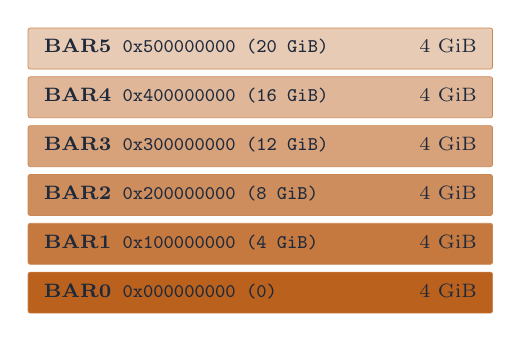
\begin{tikzpicture}[font=\scriptsize, node distance=0.9mm,
    dmabar/.style={rectangle, draw=cDmaP!70, line width=0.25pt,
                   rounded corners=0.8pt, inner xsep=2mm, inner ysep=1.2mm,
                   text=cInk}]
  % highest region first; each row hangs below the previous one
  \node[dmabar, fill=cDmaP!30]                    (bar5) {\dmarow{BAR5}{0x500000000 (20 GiB)}};
  \node[dmabar, fill=cDmaP!42, below=of bar5]     (bar4) {\dmarow{BAR4}{0x400000000 (16 GiB)}};
  \node[dmabar, fill=cDmaP!54, below=of bar4]     (bar3) {\dmarow{BAR3}{0x300000000 (12 GiB)}};
  \node[dmabar, fill=cDmaP!66, below=of bar3]     (bar2) {\dmarow{BAR2}{0x200000000 (8 GiB)}};
  \node[dmabar, fill=cDmaP!78, below=of bar2]     (bar1) {\dmarow{BAR1}{0x100000000 (4 GiB)}};
  \node[dmabar, fill=cDmaP!92, below=of bar1]     (bar0) {\dmarow{BAR0}{0x000000000 (0)}};
\end{tikzpicture}
\end{center}
\note{DMA 用 64 位偏移访问，配合 \lit{-A} 使用；BAR 侧的 \lit{-i} 只在单个 BAR 内计算偏移。}
\end{panel}

% ------------------------------------------------------------ THREAD MAP
\begin{panel}{cDma}{\lit{-Y} / \lit{-Z} 线程与 BAR0 区域分配}
\begin{center}
\begin{tikzpicture}[font=\scriptsize, node distance=0.45mm,
    tblk/.style={rectangle, draw=cDma!70, line width=0.25pt, align=center,
                 minimum width=9.4mm, minimum height=10mm, inner sep=0.6mm,
                 text=cInk},
    addr/.style={font=\ttfamily\tiny, text=cGrey}]
  % cells run left to right, each hooked onto the previous one
  \node[tblk, fill=cDma!85]                  (t1) {\bfseries\#1\\\ttfamily 0x77};
  \node[tblk, fill=cDma!73, right=of t1]     (t2) {\bfseries\#2\\\ttfamily 0x88};
  \node[tblk, fill=cDma!61, right=of t2]     (t3) {\bfseries\#5\\\ttfamily 0xBB};
  \node[tblk, fill=cDma!49, right=of t3]     (t4) {\bfseries\#3\\\ttfamily 0x99};
  \node[tblk, fill=cDma!37, right=of t4]     (t5) {\bfseries\#4\\\ttfamily 0xAA};
  \node[tblk, fill=cDma!27, right=of t5]     (t6) {\bfseries\#6\\\ttfamily 0xCC};
  \node[tblk, fill=cDma!18, right=of t6]     (t7) {\bfseries\#7\\\ttfamily 0xDD};

  % offset labels hang under their own cell
  \node[addr, below=1.2mm of t1] (a1) {0};
  \node[addr, below=1.2mm of t2] (a2) {1024};
  \node[addr, below=1.2mm of t3] (a3) {2048};
  \node[addr, below=1.2mm of t4] (a4) {3072};
  \node[addr, below=1.2mm of t5] (a5) {4096};
  \node[addr, below=1.2mm of t6] (a6) {5120};
  \node[addr, below=1.2mm of t7] (a7) {6144};

  % the ruler spans from the left edge of the first cell to the right edge of the last
  \draw[cGrey, line width=0.3pt]
        (a1.south -| t1.west) -- (a7.south -| t7.east);
  \node[below=1mm of a4, font=\tiny, text=cGrey] {BAR0 偏移（每格 1 KiB）};
\end{tikzpicture}
\end{center}
\note{注意 \#5 落在 2048、\#3 落在 3072，线程号与地址顺序\textbf{并不一致}。}
\end{panel}

% ------------------------------------------------------------ EXEC ORDER
\begin{panel}{cMisc}{任务执行顺序（选项模式）}
{\scriptsize 多个任务被合并成一个 action 位图，按\textbf{枚举位序}执行，
\textcolor{cWarn}{与命令行书写顺序无关}。\par}
\vspace{1.5mm}
\begin{center}
\begin{tikzpicture}[font=\tiny,node distance=1.6mm,
    st/.style={rectangle,rounded corners=1.6pt,fill=#1!15,draw=#1!60,
               text=cInk,inner xsep=3pt,inner ysep=2.2pt,align=center}]
  \node[st=cBar] (s1) {BAR 读 / 写\\ 单点写 / 单点读 / 查大小};
  \node[st=cDma,below=of s1] (s2) {DMA 读 / 写\\ SG 事件 / 中断 / 唤醒};
  \node[st=cMisc,below=of s2] (s3) {驱动版本};
  \node[st=cBarP,below=of s3] (s4) {BAR ioctl 读写测试\\ BAR mmap 读 / 写 / 读写测试};
  \node[st=cDmaP,below=of s4] (s5) {DMA mmap 测试 / 扫描 / 初始化\\ 用户态 DMA / 多线程 读 写 循环};
  \node[st=cEx,below=of s5] (s6) {SG 描述符长度 / 系统时钟\\ FIFO 读 / FIFO 写};
  \foreach \a/\b in {s1/s2,s2/s3,s3/s4,s4/s5,s5/s6}
     \draw[-{Stealth[length=3pt]},cGrey] (\a) -- (\b);
\end{tikzpicture}
\end{center}
\note{所以 \lit{-j 0 -c 0 -h 8 -k 0x55} 会\textbf{先写后读}，而不是按字面顺序。}
\note{\textcolor{cWarn}{\bfseries 陷阱：}\lit{-t} 和 \lit{-u} 用的是赋值而非按位或，
      会\textbf{清掉之前累积的所有任务}。混用时把它们放最前面。}
\end{panel}

% ------------------------------------------------------------ NUMERIC MODE
\begin{panel}{cNum}{编号模式：测试编号与位置参数}
{\scriptsize 下标约定：\lit{[1]} I/O 设备序号 · \lit{[2]} DMA 设备序号 · \lit{[3]} 测试编号。
\lit{--help} 打印的列表按数组顺序输出，\textbf{显示顺序不等于编号顺序}。\par}
\vspace{1mm}
\testrow{0}{BAR：ioctl 读}{[4] BAR 0-5 · [5] 长度 <=1048576 · [6] 偏移 <=1048576}
\testrow{1}{BAR：ioctl 写}{[4] BAR · [5] 长度 · [6] 偏移 · [7] 1=定值/0=随机 · [8] 定值 0-255}
\testrow{2}{BAR：ioctl 写后回读}{[4] BAR · [5] 长度 · [6] 偏移}
\testrow{3}{DMA：ioctl 读（设备→主机）}{[4] 通道 0-6 · [5] 偏移 · [6] 长度 · [7] 0=direct/1=SG · [8] 0=非阻塞/1=阻塞 · [9] 0=递增/1=固定}
\testrow{4}{DMA：ioctl 写（主机→设备）}{[4]-[9] 同上 · [10] 1=定值/0=随机 · [11] 定值 0-255}
\testrow{5}{DMA：ioctl 读写循环}{[4]-[9] 同 ID 3 · [10] 循环次数（0 = 无限）}
\testrow{6}{BAR：mmap 读}{[4] BAR · [5] 长度 · [6] 偏移}
\testrow{7}{BAR：mmap 写}{[4] BAR · [5] 长度 · [6] 偏移 · [7] 1=定值/0=随机 · [8] 定值}
\testrow{8}{BAR：mmap 写后回读}{[4] BAR · [5] 长度 · [6] 偏移}
\testrow{9}{BAR：mmap 读写循环}{[4] BAR · [5] 长度 · [6] 偏移 · [7] 循环次数}
\testrow{10}{BAR：pread（read+lseek）读}{[4] BAR · [5] 长度 · [6] 偏移}
\testrow{11}{BAR：pwrite（write+lseek）写}{[4] BAR · [5] 长度 · [6] 偏移 · [7] 1=定值/0=随机 · [8] 定值}
\testrow{12}{BAR：read/write/lseek 读写组合}{[4] BAR · [5] 长度 · [6] 偏移 · [7] 1=定值/0=随机 · [8] 定值}
\testrow{13}{BAR：多线程读写}{[4] 线程数 1-20 · [5] 循环上限（0=无限） · [6] 起始偏移（默认 0） · [7] 总长度（默认 2048，1-1048576）}
\testrow{14}{DMA：多通道多线程读写}{[4] 线程数 <=7 · [5] 循环上限（0=无限） · [6] 起始偏移（默认 0） · [7] 总长度（默认 2048） · [8] 阻塞模式（默认 1）}
\testrow{15}{DMA 多线程 + 8 个 BAR ioctl 线程}{[4] 循环上限 · [5] BAR 偏移（0） · [6] BAR 总长（16384） · [7] DMA 偏移（0xC000=49152） · [8] DMA 总长（16384） · [9] 阻塞模式（1）}
\testrow{16}{BAR + DMA 组合线程测试}{无位置参数；固定 8 个 BAR 线程 + 7 个 DMA 线程}
\sep
{\scriptsize
$\bullet$\ \textbf{测试 0--13}：参数缺失逐项交互提问；超范围直接报错退出。\par
$\bullet$\ \textbf{测试 14--16}：不提问，缺失即取默认值；线程数超 7 告警并回退。\par
$\bullet$\ \textbf{测试 15、16} 不在 \lit{--help} 列表里，但可正常指定。\par
$\bullet$\ \textcolor{cWarn}{\textbf{测试 5}} 要求驱动 commit \textbf{>= 239}；更早版本在 SG 模式下约 200 万次后
会因内存泄漏和 page unpin 丢失而失败，FPGA 固件也须支持带偏移/长度的区域读写。\par
$\bullet$\ 测试 13/14/15 启动时会先打印自己的参数格式，可直接照抄。\par}
\end{panel}

% ------------------------------------------------------------ SIGNALS
\begin{panel}{cMisc}{运行期信号}
\cmdrow{cMisc}{SIGINT}{Ctrl+C}{}{置停止标志，通知所有 BAR / DMA 线程收尾退出}
\cmdrow{cMisc}{SIGUSR1}{}{}{立即打印所有 BAR / DMA 线程的统计信息}
\cmdrow{cMisc}{SIGUSR2}{}{}{切换 BAR / DMA 线程的 verbose 日志开关}
\note{跑无限循环时用 \lit{kill -USR1 <pid>} 观察进度，\lit{Ctrl+C} 收尾。}
\end{panel}

% ------------------------------------------------------------ NUMBER FORMAT
\begin{panel}{cMisc}{数值格式约定}
{\scriptsize
\textcolor{cEx}{\bfseries 支持 0x 前缀}（否则十进制）：\par
\vspace{0.6mm}
\lit{-l}\ \ \lit{-i}\ \ \lit{-h}\ \ \lit{-k}\ \ \lit{-L}\ \ \lit{-A}\ \ \lit{-K}\ \ \lit{-S}\ \ \lit{-I}\par
\vspace{1.4mm}
\textcolor{cWarn}{\bfseries 只按十进制解析}（写 \lit{0x10} 会被解析成 0）：\par
\vspace{0.6mm}
\lit{-j}\ \ \lit{-c}\ \ \lit{-g}\ \ \lit{-m}\ \ \lit{-n}\ \ \lit{-C}\ \ \lit{-B}\ \ \lit{-H}\ \ \lit{-J}\ \ \lit{-E}\ \ \lit{-G}\ \ \lit{-U}\ \ \lit{-F}\ \ \lit{-b}\ \ \lit{-e}\ \ \lit{-s}\par
\vspace{1.4mm}
编号模式的所有位置参数\textbf{只接受十进制非负整数}，不支持 \lit{0x}。\par}
\end{panel}

% ------------------------------------------------------------ EXAMPLES
\begin{panel}{cEx}{常用命令示例}
{\scriptsize 下文用 \lit{IO=/dev/GOOGOL\_PCIe\_x86\_64\_io\_0}、
\lit{DMA=/dev/GOOGOL\_PCIe\_x86\_64\_dma\_0} 代指。\par}
\vspace{1mm}
{\color{cEx}\bfseries\scriptsize BAR 读写}
\shell{pci_test -d $IO -r 0}
\shell{pci_test -d $IO -r 0 -l 2048 -i 2048}
\shell{pci_test -d $IO -w 0 -l 2048 -i 20 -k 0xAA}
\shell{pci_test -d $IO -c 0 -h 8 -k 0x55AA -a short}
\shell{pci_test -d $IO -j 0 -h 8 -a short}
\shell{pci_test -d $IO -t 0 -l 2048}
\shell{pci_test -d $IO -u 0 -l 2048}
\shell{pci_test -d $IO -g 0}
\vspace{1.2mm}
{\color{cEx}\bfseries\scriptsize FPGA FIFO}
\shell{pci_test -d $IO -b 1024}
\shell{pci_test -d $IO -e 2048}
\vspace{1.2mm}
{\color{cEx}\bfseries\scriptsize DMA 读写}
\shell{pci_test -D $DMA -W -A 0 -L 2048 -O 0}
\shell{pci_test -D $DMA -W -A 0 -L 2048 -K 0xAA -O 1}
\shell{pci_test -D $DMA -W -A 0 -L 2048 -O 1 -H 1}
\shell{pci_test -D $DMA -R -A 1024 -L 2048 -C 2 -O 1}
\shell{pci_test -D $DMA -E 0}
\shell{pci_test -D $DMA -T}
\shell{pci_test -D $DMA -F 4096}
\vspace{1.2mm}
{\color{cEx}\bfseries\scriptsize 多线程压测}
\shell{pci_test -d $IO -D $DMA -X}
\shell{pci_test -d $IO -D $DMA -Y}
\shell{pci_test -d $IO -D $DMA -Z}
\shell{pci_test 0 0 13 8 0 0 2048}
\shell{pci_test 0 0 14 7 0 0 2048 1}
\shell{pci_test 0 0 15 0 0 16384 49152 16384 1}
\vspace{1.2mm}
{\color{cEx}\bfseries\scriptsize 版本与帮助}
\shell{pci_test --version}
\shell{pci_test -d $IO -p}
\shell{pci_test -D $DMA -P}
\shell{LANG=zh_CN.UTF-8 pci_test --help}
\shell{LANG=C pci_test --help}
\end{panel}

% ------------------------------------------------------------ PITFALLS
\begin{panel}{cWarn}{已知不一致 / 使用陷阱}
{\scriptsize 以下都是源码层面的实际情况，与内置 \lit{--help} 文本对不上，以本卡为准。\par}
\vspace{1mm}
{\scriptsize
\textcolor{cWarn}{\bfseries 1.}\ \lit{-N} / \lit{--dma\_mmap\_write} \textbf{不可用}。
它同时出现在短选项串和长选项表里，但 switch 缺对应分支，会落到 default 报
\lit{unknown options}，导致整个解析失败。\par\vspace{1mm}
\textcolor{cWarn}{\bfseries 2.}\ \lit{--fifo\_read\_test} / \lit{--fifo\_write\_test}
\textbf{长选项形式不可用}：长选项表声明为 no\_argument，代码却要求 optarg。
只能用 \lit{-b} / \lit{-e}。\par\vspace{1mm}
\textcolor{cWarn}{\bfseries 3.}\ \lit{-G} 与 \lit{-U} 的\textbf{长选项名与行为互换}：
\lit{--wakeup\_dma} 查中断状态，\lit{--get\_dma\_interrupt\_status} 做唤醒。\par\vspace{1mm}
\textcolor{cWarn}{\bfseries 4.}\ 帮助里的长选项名过时：\lit{-M} 写作 \lit{--mapped\_direct\_dma\_test}，
实际是 \lit{--dma\_mmap\_read}；\lit{-A} 写作 \lit{--dma\_access\_address}，
实际是 \lit{--dma\_access\_offset}。\par\vspace{1mm}
\textcolor{cWarn}{\bfseries 5.}\ \lit{-g}、\lit{-s}、\lit{-I} \textbf{未出现在 \lit{--help} 输出里}，但都可用。\par\vspace{1mm}
\textcolor{cWarn}{\bfseries 6.}\ \lit{-a int} 不被接受，尽管帮助以它举例。32 位请用
\lit{4} / \lit{int32} / \lit{uint32} / \lit{int32\_t}。\par\vspace{1mm}
\textcolor{cWarn}{\bfseries 7.}\ \textbf{BAR 号解析静默降级}：\lit{-r/-w/-t/-u} 遇到
\lit{bar 0}、\lit{06}、\lit{BAR6} 等不报错，一律当 BAR0。\par\vspace{1mm}
\textcolor{cWarn}{\bfseries 8.}\ \textbf{测试编号上界差一}：校验允许输入 17，但有效编号只有 0--16，
17 会走到 default 报 \lit{Unknown test id specified}。\par\vspace{1mm}
\textcolor{cWarn}{\bfseries 9.}\ 编号模式的设备扫描\textbf{写死 x86\_64 命名}
（\lit{GOOGOL\_PCIe\_x86\_64\_io*} / \lit{...\_dma*}）。其他架构上编号模式找不到设备，
请改用选项模式并用 \lit{-d} / \lit{-D} 直接给路径。\par\vspace{1mm}
\textcolor{cWarn}{\bfseries 10.}\ \textbf{两种模式的显示格式默认值不同}：选项模式默认十进制（显示偏移），
编号模式解析时会把选项结构体重新清零，默认变成十六进制（显示绝对地址）。\par\vspace{1mm}
\textcolor{cWarn}{\bfseries 11.}\ \lit{-t} / \lit{-u} \textbf{会清空之前累积的任务}，见「任务执行顺序」。\par}
\end{panel}

\end{multicols}
\end{document}
